\chapter{Convex Learning Problems}
\chapterauthor{Samuel Ireson}

\begin{chout}
	Another common method of limiting the hypothesis space is by asserting it to be convex. We will explore learning problems in this area in the following chapter, encountering some challenging associated concepts.
\end{chout}

\section{Convexity}

\begin{definition}[Convex set]
	A set $ C $ is said to be \defined{convex} if for every pair of points $ a,b \in C $, the following inclusion holds,
	\begin{align*}
		\{ \lambda a + (1- \lambda) b: \lambda \in [ 0,1 ] \} \subseteq C
	\end{align*}
\end{definition}

There is a good geometric intuition for this definition. In particular, the set which must be included in $ C $ describes the straight line from $ a $ to $ b $. So, a set $ C $ is convex if and only if it contains every straight line between any two points. See the figure below.

\begin{figure}[!htb]
	\centering
	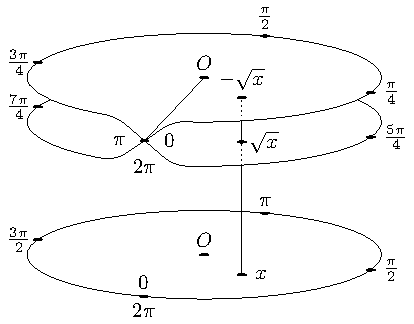
\includegraphics{convex-sets/figure.pdf}
	\caption{The set $ C $ is convex, but since we can find a line which is not contained in the set $ N $, this set is not convex.}
\end{figure}
